% BEGIN (PARALLELISATION)
% ===========================================================================
\subsection{Overview}

Within a FLAME simulation, every agent only interacts with its environment via the reading and writing of messages to a collection of Message Boards. This makes the Message Board component an ideal candidate for enabling parallelism. 

Using distributable Message Boards, agents can be farmed out across multiple processing nodes and simulated in parallel while coherency of the simulation is maintained through the unified view of the distributed Boards.

\begin{figure}[h]
 \centering
  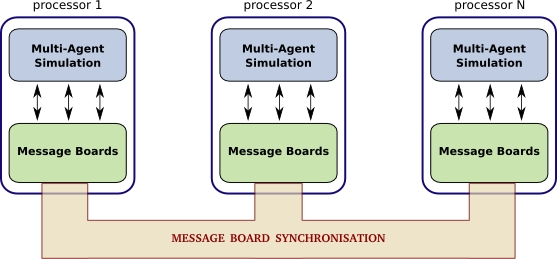
\includegraphics[scale=0.50]{mboard_flame.jpg}
 \caption{Parallelisation of FLAME using distributed Message Boards}
 \label{fig:mb_flame}
\end{figure}

\subsection{The Message Board library}
In the recent code release, the Message Board was decoupled from the FLAME framework and implemented as a separate library. This provides us with the flexibility to experiment with different parallelisation strategies while minimising the impact on current users of the FLAME framework.

\begin{figure}[h]
 \centering
  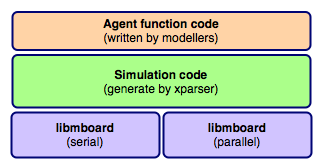
\includegraphics[scale=0.60]{mboard_overview.png}
 \caption{Users can create either serial or parallel executables by linking their object files to the appropriate \textit{libmboard} library}
 \label{fig:mb_overview}
\end{figure}

The Message Board Library (\textit{libmboard}) can be built as a set of static libraries which can be linked to users' simulation object files to create serial and parallel executables. This setup enables users to maintain a common source base for both serial and parallel simulations, thus simplifying code management and testing. It will also provide \textit{libmboard} developers the facility to quickly switch between different library implementations without having to continuously recompile the test program.

All functionalities provided by the Message Board Library is accessible via the \textit{libmboard} Application Program Interface (API). Through the API, users interface only with the provided routines and a set of opaque datatypes, providing them access to the functionality of the library while requiring any notion of the internal implementation. The complete communication strategy and data representation system can be replaces without any users. This flexbility is crucial in the EURACE project as \textit{libmboard} is being developed in tandem with modelling activities that require a working implementation.


Within the FLAME framework, the \textit{libmboard} API is used within routines generated by the framework and not directly by the modellers. Modellers are provided with model-specific routines that hides to complexity of managing boards and packaging data into suitable datatypes. Figure~\ref{fig:mb_api_flame} provides and example of this whereby an agent's message add request gets translated to a \textit{libmboard} API call.
\begin{figure}[h]
 \centering
  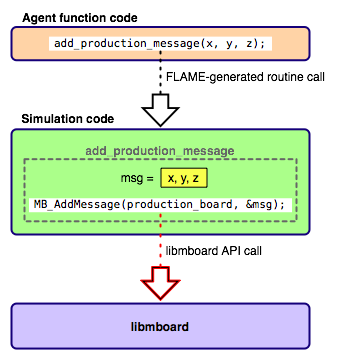
\includegraphics[scale=0.60]{mboard_codetranslate.png}
 \caption{Modellers use FLAME-generated routines which gets translated to the appropriate \textit{libmboard} API call}
 \label{fig:mb_api_flame}
\end{figure}

\textit{libmboard} uses MPI to communicate between processors, and POSIX threads (pthreads) to manage a separate thread for handling data management and inter-process communication. Futher details are available in Section~\ref{sec:mb_sync} and Section~\ref{sec:commthread}.

% ===========================================================================
\subsection{The \textit{libmboard} API}
\label{sec:mb_api}

%\begin{itemize}
%\item Quick desc of the API. Point to User Doc for details.
%\item Opaque objects
%\item return codes
%\end{itemize} 

The  \textit{libmboard} API is intended for use within the FLAME generated simulation code. It provides the functionality for creating, managing and accessing Message Boards. Implementation details such as internal data representations, memory management and communication strategies are transparent to API users and therefore can be replaced or improved without affecting FLAME developers and end-users.

In this following sections, we discuss the use of Boards, Iterators and Synchronisation. For further details, refer to the \textit{libmboard} Reference Manual\cite{MessageBoardAPI} which includes the full API specification and usage example.
% ---------------------------------------------------------------------------
%\subsubsection{Library environment}

%\begin{itemize}
%\item Init and finalise
%\item MPI env
%\item fork/join comm thread thread
%\end{itemize} 

% ---------------------------------------------------------------------------
\subsubsection{Boards}

Message Boards are essentially distributed data structures that can be read and written to by agents on all processing nodes. Up to 4096 different Message Boards can be created, whereby each Board is created to store message objects of a specified size.

Message Boards are created using the \texttt{MB\_Create()} routine. This routine will return a Board Handle (of type \texttt{MBt\_Board}) which can be used to reference the Board when performing further operations on the Board.

Once a Board is created, messages can be added to it using the \texttt{MB\_AddMessage()} routine. During an add, the message data is copied and store in Board, allowing the calling code to reuse or deallocate the original message data. The cloning of data greatly simplifies the usage of the API and protects the internal data representation from accidental corruption. 

Messages added to the Board are immediately available to all agents within the local processing node, or after a sync (see Section~\ref{sec:mb_sync}), across all processing nodes.

The API provides further routines from emptying (\texttt{MB\_Clear()}) and deleting  (\texttt{MB\_Delete()}) Boards.

% ---------------------------------------------------------------------------
\subsubsection{Iterators}
\label{sec:mb_interators}

Iterators provides the calling code with a mechanism for traversing Message Board content. 
\begin{itemize}
\item isolate users from internal data representation
\item normal/filtered/sorted
\item returning cloned mem vs ptr.
\item randomisation
\item rewind
\end{itemize} 

% ---------------------------------------------------------------------------
\subsubsection{Synchronisation}
\label{sec:mb_sync}

\begin{itemize}
\item Message Tagging vs Filtered Iterators.
\item Why important? Impact on solution time?
\item Details on how messages are packed and distributed
\end{itemize} 

\begin{figure}[h]
 \centering
  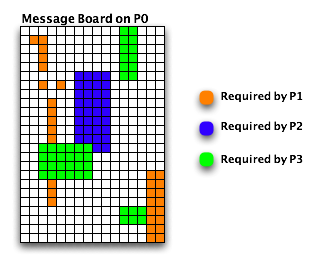
\includegraphics[scale=0.70]{taggedboard.png}
 \caption{Lorem ipsum dolor sit}
 \label{fig:taggedboard}
\end{figure}

When synchronisation of a board is requested, the board is locked and added into the \textit{Sync Queue}. Control is then returned to the the calling code, allowing it to perform other tasks that does not require access to the board being synchronised. 

The sequence diagram in  Figure~\ref{fig:syncboard} depicts how a board synchronisation request may take place. The process of actually synchronising and unlocking the board is performed concurrently in the background by the \textit{Communication Thread}. This is discussed further in Section~\ref{sec:commthread}.

\begin{figure}[h]
 \centering
  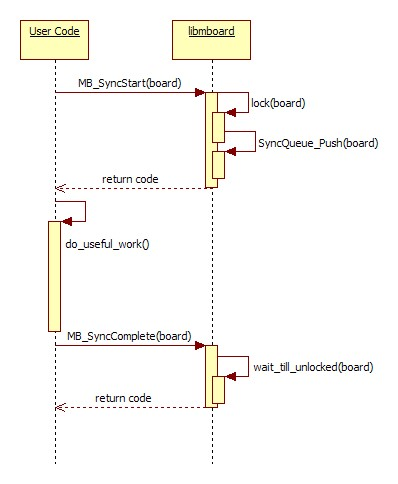
\includegraphics[scale=0.60]{syncboard.jpg}
 \caption{Other work can be schedule during board synchronisation to shadow the overheads of communication}
 \label{fig:syncboard}
\end{figure}

% ===========================================================================
\subsection{The Communication Thread}
\label{sec:commthread}

During the initialisation of the Message Board environment, \textit{libmboard} forks a \textit{Communication Thread} to handle the synchronisation of distributed boards. 

Apart from potentially making better use of multi-core processors, delegating communication and memory intensive operations to a separate thread also allows us to minimise the effective overheads by performing them concurrently with the main simulation and thus overlapping the Board synchronisation time with that of useful computation.

To simplify thread-safety, the \textit{Communication Thread} interacts with the main thread mainly through the \textit{Sync Queue} and the locking mechanism of each board. Access to these components are protected by mutex locks provided by \textit{pthreads} API. Boards that need to be synchronised are locked by the main thread and pushed into the \textit{Sync Queue}. The \textit{Communication Thread} indicate the completion of a synchronisation process by unlocking the board.

\begin{itemize}
\item motivation
\item queues
\end{itemize} 



\begin{figure}[h]
 \centering
  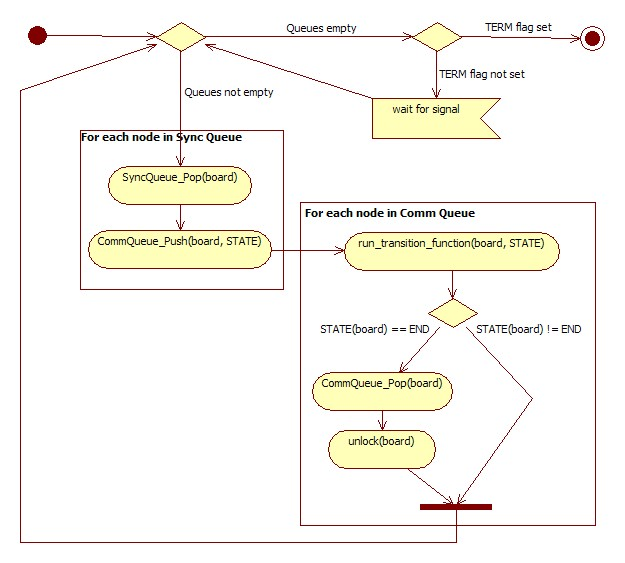
\includegraphics[scale=0.50]{commloop.jpg}
 \caption{Activity diagram for Communication Thread}
 \label{fig:commloop}
\end{figure}

\begin{figure}[h]
 \centering
  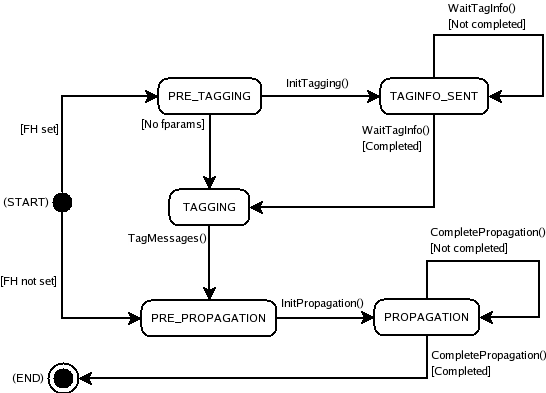
\includegraphics[scale=0.50]{CommNode.png}
 \caption{State diagram for processing Communication Node}
 \label{fig:commstate}
\end{figure}

% ===========================================================================
\subsection{Issues}

\begin{itemize}
\item Synchronising handles (boards, iterators, functions). Checking = Blocking operations = large overheads. Use debug v production.
\item MPI thread support
\item Job scheduling more complex if consider threads
\item MPI sends/receives requires contiguous buffers. Expensive (space and time) packing of messages.
\item Comm stages not fully non-blocking
\item Total tagged messages may be more than actual message. Gets works with more proc. Scaling issues.
\item Filters not widely used (or even fully implemented in FLAME)
\end{itemize} 

% ===========================================================================
